\documentclass{beamer}

\mode<presentation> {

\usetheme{CambridgeUS}
\usepackage[spanish]{babel}
\usepackage{graphicx} % Allows including images
\usepackage{multimedia}
\usepackage[autosize]{dot2texi}
\usepackage{tikz}
\usepackage{amsmath}
\usetikzlibrary{shapes,arrows}


\AtBeginSection[]{
  \begin{frame}
  \vfill
  \centering
  \begin{beamercolorbox}[sep=8pt,center,shadow=true,rounded=true]{title}
    \usebeamerfont{title}\insertsectionhead\par%
  \end{beamercolorbox}
  \vfill
  \end{frame}
}

%\setbeamertemplate{footline} % To remove the footer line in all slides uncomment this line
\setbeamertemplate{footline}[page number] % To replace the footer line in all slides with a simple slide count uncomment this line

\setbeamertemplate{navigation symbols}{} % To remove the navigation symbols from the bottom of all slides uncomment this line
}

\usepackage{booktabs} % Allows the use of \toprule, \midrule and \bottomrule in tables
%----------------------------------------------------------------------------------------
%	TITLE PAGE
%----------------------------------------------------------------------------------------

\title[Short title]{Trabajo Práctico Nro. 2: Autómatas Celulares} % The short title appears at the bottom of every slide, the full title is only on the title page

\author{
  \texorpdfstring{Leandro Ezequiel Rodriguez}{Leandro Ezequiel Rodriguez}\\
  \texorpdfstring{Gaspar Budó Berra}{Gaspar Budó Berra}\\
  \texorpdfstring{Juan Martin Barmasch}{Juan Barmasch}
}
\institute[ITBA] % Your institution as it will appear on the bottom of every slide, maybe shorthand to save space
{
Instituto Tecnológico de Buenos Aires \\ % Your institution
\medskip
\textit{\{learodriguez, jbarmasch, gbudoberra\}@itba.edu.ar} % Your email
}
\date{\Today} % Date, can be changed to a custom date

\useoutertheme[subsection=false]{miniframes}
\begin{document}

\begin{frame}
\titlepage % Print the title page as the first slide
\end{frame}

% \begin{frame}
% \frametitle{Overview} % Table of contents slide, comment this block out to remove it
%\tableofcontents % Throughout your presentation, if you choose to use \section{} and \subsection{} commands, these will automatically be printed on this slide as an overview of your presentation
% \end{frame}

%----------------------------------------------------------------------------------------
%	PRESENTATION SLIDES
%----------------------------------------------------------------------------------------

%------------------------------------------------
\section{Introducción}
%------------------------------------------------

\subsection{}
\begin{frame}
\frametitle{Introducción}
\indent{Se presentará un trabajo de análisis de sistemas de bandadas de agentes autopropulsados, utilizando un autómata de espacio no discretizado conocido como Off-Lattice.}
\end{frame}


\subsection{}
\begin{frame}
\frametitle{Off-Lattice}
Reglas del autómata:
\begin{center}
    \begin{align}
        x_i(t+1)=x_i(t)+v_i(t)\Delta t\\
        \theta(t+1)=\langle\theta(t)\rangle_r+\Delta\theta
    \end{align}
    \begin{itemize}
        \item[$\ast$] $x_i(t)$: posición del agente i en el instante t
        \item[$\ast$] $v_i(t)$: velocidad del agente i en el instante t
        \item[$\ast$] $\langle\theta(t)\rangle_r$: promedio de los angulos de todos los agentes dentro de r
        \item[$\ast$] $\Delta\theta$: ruido uniforme en el rango $[\frac{\eta}{2},\frac{\eta}{2}]$
    \end{itemize}
    \end{center}
\end{frame}
% A subsection can be created just before a set of slides with a common theme to further break down your presentation into chunks

%------------------------------------------------
\section{Implementacion}

\subsection{Arquitectura}
\begin{frame}{Arquitectura: UML}
\begin{figure}[h]
    \centering
    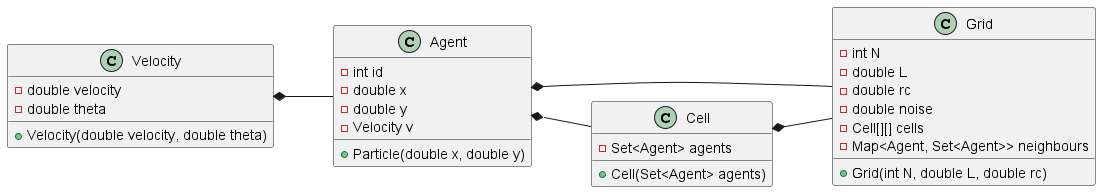
\includegraphics[width=1\textwidth]{images/tp2models.png}
  \end{figure}

\end{frame}


%------------------------------------------------
\section{Simulaciones}

\begin{frame}{Parametros}
    \begin{enumerate}
        \item[1] $\rho$: Densidad de la simulación $(\frac{N}{L^2})$
        \item[2] $\eta$: Ruido aportado al calculo de los ángulos
        \item[3] $v$: Módulo de la velocidad ($cte=0.03$)
    \end{enumerate}
\end{frame}

\begin{frame}{Variable a analizar}
    \begin{itemize}
        \item[$\ast$] Parámetro de orden:
    \end{itemize}
    \begin{center}
        \begin{align}
            v_a=\frac{1}{N_v}|\sum\limits^{N}_{i=1} v_i|
        \end{align}
        \begin{enumerate}
            \item[$\ast$] Mide el estado de polarización de los agentes
                \begin{enumerate}
                    \item[i] Completo desorden: $v_a\rightarrow 0$
                    \item[ii] Completa polarización: $v_a\rightarrow 1$
                \end{enumerate}
        \end{enumerate}
    \end{center}
\end{frame}

\subsection{Simulaciones-A}
\begin{frame}{Simulación A-I}

\frametitle{Simulación A: Primera Parte}
\end{frame}

\begin{frame}{Simulación A-II}

\frametitle{Simulación A: Segunda Parte}
\end{frame}

\subsection{Simulaciones-B}
\begin{frame}{Simulación B-I}

\frametitle{Simulación B: Primera Parte}
\end{frame}

\begin{frame}{Simulación B-II}

\frametitle{Simulación B: Segunda Parte}
\end{frame}


%------------------------------------------------
\section{Resultados}

\subsection{Resultados}
\begin{frame}{Resultados}

\end{frame}

%-----------------------------------------------
\section{Conclusiones}
\subsection{Conclusiones}
\frametitle{Conclusiones}
\begin{frame}{Conclusiones}
\begin{itemize}
    \item[1] Conclusión 1
    \item[2] Conclusión 2
\end{itemize}
\end{frame}

\begin{frame}
\Huge{\centerline{Muchas gracias}}
\end{frame}

%----------------------------------------------------------------------------------------

\end{document}